\documentclass[a4paper]{article}
\usepackage{Sweave}

%\VignetteIndexEntry{randomLCA Example}

\begin{document}


\section{Introduction}

This example shows the fitting of the dentistry data from Qu, Tan and Kutner (1996). The data consists of the results of five dentists evaluating x-rays for presence or absence of caries. As there is no gold standard, the latent class method is to assume two classes, diseased and non-diseased which are identified from the data.

\section{Latent Class}

A series of latent class models for 1 to 4 classes can be fitted using the commands
\begin{Schunk}
\begin{Sinput}
> dentistry.lca1 <- randomLCA(dentistry[, 1:5], 
+     freq = dentistry$freq, nclass = 1)
> dentistry.lca2 <- randomLCA(dentistry[, 1:5], 
+     freq = dentistry$freq, nclass = 2)
> dentistry.lca3 <- randomLCA(dentistry[, 1:5], 
+     freq = dentistry$freq, nclass = 3)
> dentistry.lca4 <- randomLCA(dentistry[, 1:5], 
+     freq = dentistry$freq, nclass = 4)
\end{Sinput}
\end{Schunk}

The BIC values may be extracted from the fitted objects and are shown in Table~\ref{tab:bic}. This indicates the presence of 3 classes. A possible interpretation is that there is a class of subjects with moderate disease, or the alternative of heterogeneous disease which will be covered in the next section. Outcome probabilities are shown in Figure~\ref{fig:outcome3}.

\begin{Schunk}
\begin{Sinput}
> bic.data <- data.frame(classes = 1:4, bic = c(dentistry.lca1$bic, 
+     dentistry.lca2$bic, dentistry.lca3$bic, dentistry.lca4$bic))
\end{Sinput}
\end{Schunk}




% latex table generated in R 2.6.2 by xtable 1.5-2 package
% Fri Apr  4 12:40:24 2008
\begin{table}[ht]
\begin{center}
\begin{tabular}{rr}
  \hline
classes & bic \\
  \hline
1 & 17531.1 \\
  2 & 15021.6 \\
  3 & 14962.9 \\
  4 & 15000.0 \\
   \hline
\end{tabular}
\caption{BIC by class.}
\label{tab:bic}
\end{center}
\end{table}


\begin{figure}
  \centering
\begin{Schunk}
\begin{Sinput}
> trellis.par.set(col.whitebg())
> print(plot(dentistry.lca3, type = "l", xlab = "Dentist", 
+     ylab = "Outcome Probability"))
\end{Sinput}
\end{Schunk}
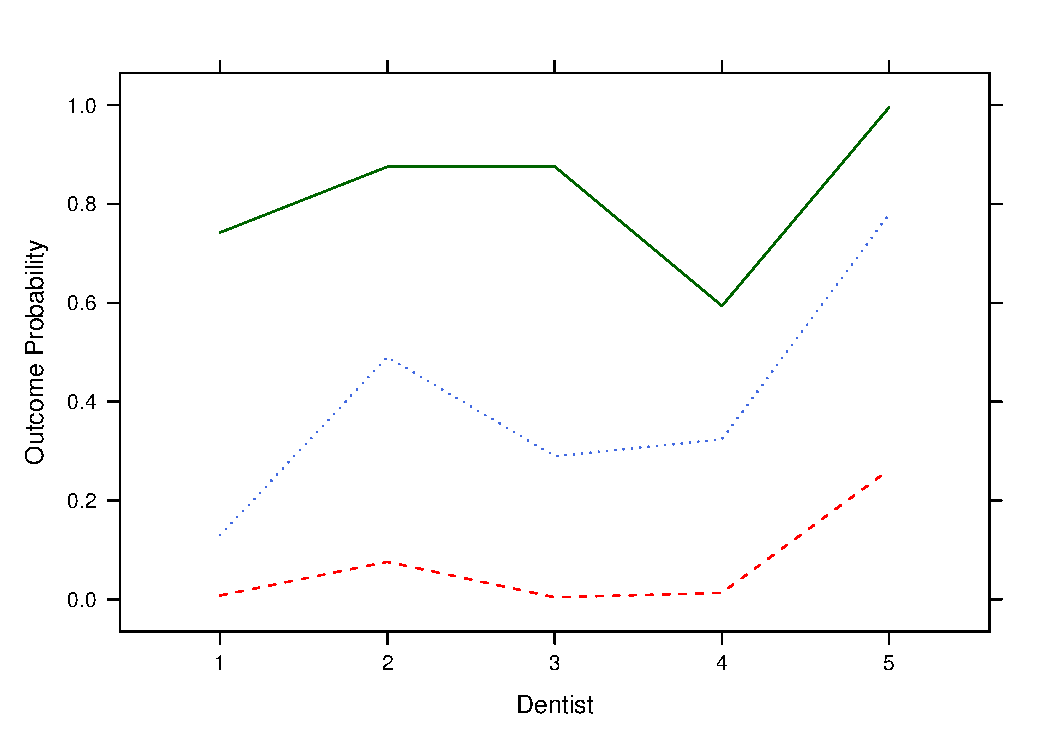
\includegraphics{randomLCA-example-input-005}
  \caption{Outcome probabilities for 3 Class Latent Class model.}
  \label{fig:outcome3}
\end{figure}

\section{Latent Class with Random Effects}

The method used in Qu, Tan and Kutner (1996) is to introduce a random effect to model heterogeneity within classes. In their model the probabilities are transformed to the probit scale and then a normal random effect introduced. In practice it usually makes little difference if a probit or logit transform is used.



\begin{Schunk}
\begin{Sinput}
> dentistry.lca2random <- randomLCA(dentistry[, 
+     1:5], freq = dentistry$freq, initmodel = dentistry.lca2, 
+     nclass = 2, random = TRUE, probit = TRUE)
\end{Sinput}
\end{Schunk}

The BIC is reduced to 14944.7 showing an improvement over any of the latent class models. An alternative model is to allow the variance of the random effect to vary by outcome (dentist). This can be performed using the \texttt{blocksize} parameter. This allows the structure of the data to be set as a series of blocks, and within each block each outcome has a different loading.

\begin{Schunk}
\begin{Sinput}
> dentistry.lca2random1 <- randomLCA(dentistry[, 
+     1:5], freq = dentistry$freq, initmodel = dentistry.lca2random, 
+     nclass = 2, random = TRUE, probit = TRUE, 
+     blocksize = 5)
\end{Sinput}
\end{Schunk}

This increases the BIC to 14949.4, and is the 2LCR model obtained by Qu, Tan and Kutner (1996). It appears that the simpler model is more appropriate.

A further extension is to allow the loading or random effect variance to vary by class. The following code will achieve that, except that the solution doesn't converge. One option is to increase the quadrature points, using \texttt{quadpoints=41} however this is insufficient here. It is simply a case of too many probabilities close to zero or one, combined with a large number of parameters compared to the number of unique observations.


\begin{verbatim}
dentistry.lca2random2 <- randomLCA(dentistry[,1:5],freq=dentistry$freq,
	initmodel=dentistry.lca2random1,nclass=2,random=TRUE,probit=TRUE,
	blocksize=5,byclass=TRUE)
\end{verbatim}


The observed and fitted values can be obtained and are shown in Table~\ref{tab:obs}. Differences from the Que et al paper result from different approximation methods.

\begin{Schunk}
\begin{Sinput}
> obs.data <- data.frame(dentistry.lca2random1$patterns, 
+     dentistry.lca2random1$observed, dentistry.lca2$fitted, 
+     dentistry.lca2random1$fitted)
> names(obs.data) <- c("V1", "V2", "V3", "V4", "V5", 
+     "Obs", "Exp 2LC", "Exp 2LCR")
\end{Sinput}
\end{Schunk}



% latex table generated in R 2.6.2 by xtable 1.5-2 package
% Fri Apr  4 12:40:47 2008
\begin{table}[ht]
\begin{center}
\begin{tabular}{rrrrrrrr}
  \hline
V1 & V2 & V3 & V4 & V5 & Obs & Exp 2LC & Exp 2LCR \\
  \hline
0 & 0 & 0 & 0 & 0 & 1880 & 1836.3 & 1882.6 \\
  0 & 0 & 0 & 0 & 1 & 789 & 830.3 & 784.7 \\
  0 & 0 & 0 & 1 & 0 & 43 & 61.9 & 38.2 \\
  0 & 0 & 0 & 1 & 1 & 75 & 49.6 & 79.7 \\
  0 & 0 & 1 & 0 & 0 & 23 & 28.6 & 24.2 \\
  0 & 0 & 1 & 0 & 1 & 63 & 47.5 & 63.8 \\
  0 & 0 & 1 & 1 & 0 & 8 & 4.0 & 6.8 \\
  0 & 0 & 1 & 1 & 1 & 22 & 35.2 & 25.8 \\
  0 & 1 & 0 & 0 & 0 & 188 & 213.9 & 184.7 \\
  0 & 1 & 0 & 0 & 1 & 191 & 152.2 & 192.5 \\
  0 & 1 & 0 & 1 & 0 & 17 & 12.1 & 23.1 \\
  0 & 1 & 0 & 1 & 1 & 67 & 61.0 & 67.2 \\
  0 & 1 & 1 & 0 & 0 & 15 & 11.2 & 12.5 \\
  0 & 1 & 1 & 0 & 1 & 85 & 91.6 & 87.4 \\
  0 & 1 & 1 & 1 & 0 & 8 & 8.1 & 7.1 \\
  0 & 1 & 1 & 1 & 1 & 56 & 86.4 & 50.8 \\
  1 & 0 & 0 & 0 & 0 & 22 & 21.2 & 18.5 \\
  1 & 0 & 0 & 0 & 1 & 26 & 25.2 & 27.9 \\
  1 & 0 & 0 & 1 & 0 & 6 & 2.1 & 4.8 \\
  1 & 0 & 0 & 1 & 1 & 14 & 16.1 & 16.0 \\
  1 & 0 & 1 & 0 & 0 & 1 & 2.5 & 2.3 \\
  1 & 0 & 1 & 0 & 1 & 20 & 24.7 & 19.7 \\
  1 & 0 & 1 & 1 & 0 & 2 & 2.2 & 1.8 \\
  1 & 0 & 1 & 1 & 1 & 17 & 23.5 & 14.5 \\
  1 & 1 & 0 & 0 & 0 & 2 & 6.0 & 7.3 \\
  1 & 1 & 0 & 0 & 1 & 20 & 42.0 & 19.8 \\
  1 & 1 & 0 & 1 & 0 & 6 & 3.7 & 4.7 \\
  1 & 1 & 0 & 1 & 1 & 27 & 39.3 & 22.4 \\
  1 & 1 & 1 & 0 & 0 & 3 & 5.7 & 2.7 \\
  1 & 1 & 1 & 0 & 1 & 72 & 61.1 & 69.6 \\
  1 & 1 & 1 & 1 & 0 & 1 & 5.4 & 3.2 \\
  1 & 1 & 1 & 1 & 1 & 100 & 58.4 & 103.0 \\
   \hline
\end{tabular}
\caption{Observed and expected frequencies}
\label{tab:obs}
\end{center}
\end{table}
The marginal outcome probabilities, obtained by integrating over the random effect can be plotted, as in Figure~\ref{fig:outcome2}.



\begin{figure}
  \centering
\begin{Schunk}
\begin{Sinput}
> trellis.par.set(col.whitebg())
> print(plot(dentistry.lca2random1, graphtype = "marginal", 
+     type = "l", xlab = "Dentist", ylab = "Marginal Outcome Probability"))
\end{Sinput}
\begin{Soutput}
NULL
\end{Soutput}
\end{Schunk}
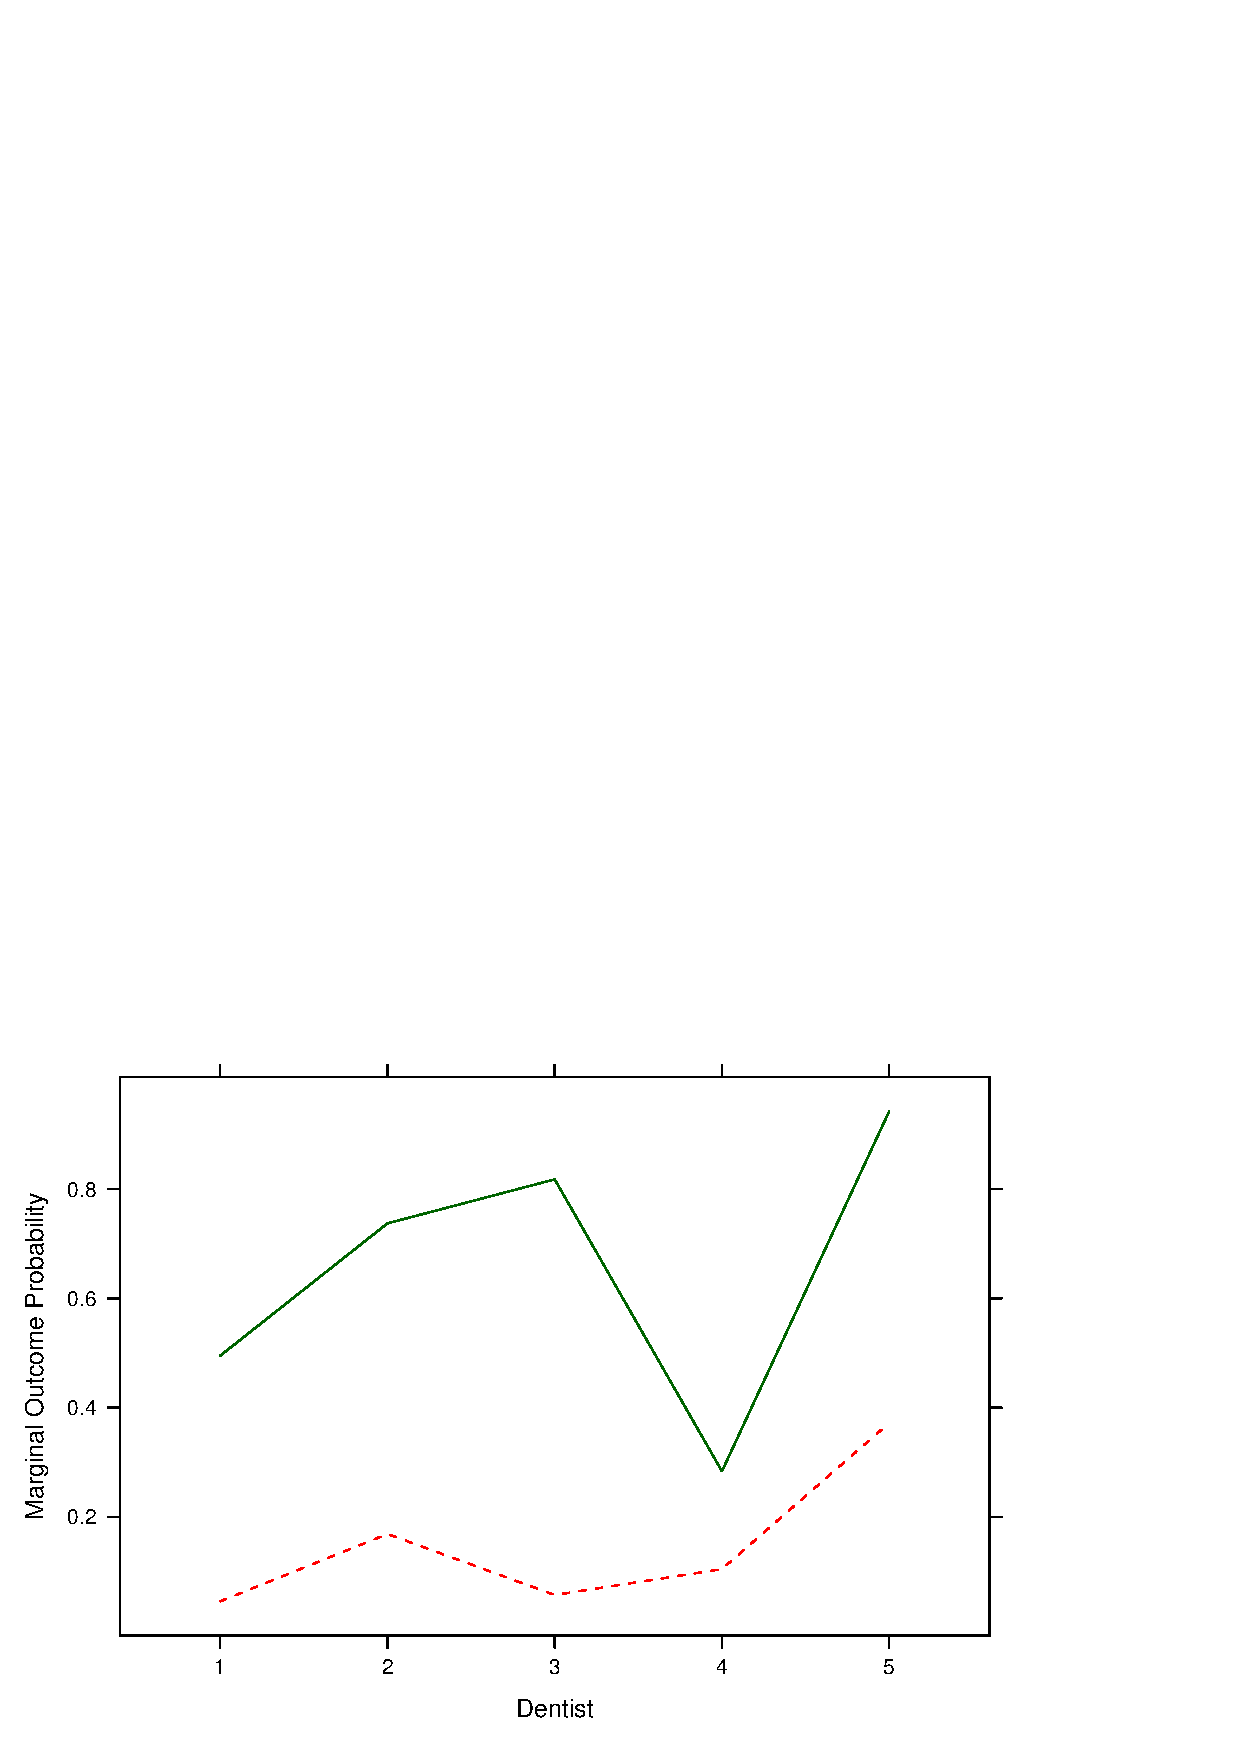
\includegraphics{randomLCA-example-input-010}
  \caption{Marginal Outcome Probabilities for 2 Class Latent Class with Random Effect (2LCR) model.}
  \label{fig:outcome2}
\end{figure}

\end{document}
